\chapter{Non-Relativistic Solution of the Hydrogen Molecular Ion in 2 Spatial Dimensions}

\section{Existing Solution s}

We apply similar method used in the 3D case of the $ H_2^{+} $ ion to find the solution in 2 dimensions. The problem itself is analogous to the 3D problem, but leads to the Mathieu's function as the solution for the radial problem.

There are not too many papers dealing with solving the $ H_2^{+} $ but here is some relevant, and recent work in this problem. In addition to the Bates paper \cite{Bates1}, there are other, more recent papers \cite{H2Plus2d1} \cite{TwoCentersParticle}, \cite{Kolos} which deal with the solution of the Schrodinger equation and spectrum of the $ H_2^{+} $ molecule.  As with other work in this problem, the paper relies on the work done by Bates et all. \cite{Bates1}. The solution in \cite{H2Plus2d1} agrees well with our solution.  One can also apply approximate methods, but they should be considered inferior to the analytical solution, we provide here. 

Analogous to the 3D case, we rely on Born-Oppenheimer (BO) approximation, in order to provide an analytical solution. The same justification for using the BO approximation in 3D molecular systems applies to the 2D problems as well, since the masses of the nuclei and electron(s) remain unchanged.  Following the same BO approximation as in Chapter 1, and using atomic units, the Schrodinger equation for the $ H_2^{+} $ molecules is given by equation \eqref{eqPartial2D} below. 

\begin{equation}\label{eqPartial2D}
\left(-\frac{1}{2}\nabla^2-\frac{1}{r_a}-\frac{1}{r_b}\right)\psi = E\,\psi
\end{equation}

The equation \eqref{eqPartial2D} is superficially similar to the equation \eqref{eqPartial3D} and the diagram \ref{h2ion3d}, but in this case, the $ r_a $ and $ r_b $ represent the nuclei coordinates in 2 dimensions.

Following the \cite{2DHAtom}, The electron wavefunction depends on only 3 quantum numbers, principal quantum number $ n $, angular quantum number $ l $ and spin $ s $. Again we ignore the spin degrees of freedom, considering the electron to be the regular 3 dimensional particles, where only its orbit is restricted to 2 dimensions.  Therefore the spin magnetic moment of the electron is not affected by the 2D restriction and the spin vector can point in any direction in 3D space. Also the orbit can have different shapes, thus there remains the need for an orbital quantum number. However, there can be one one orientation of the orbit, thus we do not consider the magnetic quantum number. This reasoning agrees with ~The solution of the electron wavefunction to the hydrogen atom in 2 dimensions \cite{H2atom} where electron wavefunction solution only depends on the principal and orbital quantum numbers.

The geometry of the 2D problem leads to choosing the elliptical coordinates (as in 3D problem), with two coordinates, $ \mu $ and $ \lambda $ denoting the position of the electron in 2D plane. \cite{Arfken}

\section{Exact solution of the electron energies of the \texorpdfstring{$ H_2^+ $}{$H_2^+$} molecule}

The goal is to provide the exact solution to the wavefunction of the $ H_2^{+} $ electron, for a given definition of exact. However even for this, relatively simple problem, it is impossible to find a closed form solution. So the solution is exact, in a sense that it can be done to an arbitrary precision.

\begin{figure}
 \captionsetup{type=figure}
  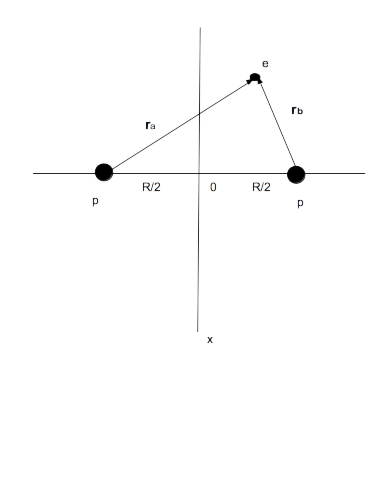
\includegraphics{H2Ion2D.png}
  \caption{Hydrogen Ion in 2 dimension} 
  \label{h2ion2d}
\end{figure}

As illustrated by the figure  \ref{h2ion2d}, we express equation \eqref{eqPartial2D} in the elliptical coordinates, and by setting the $ x $ axis to be perpendicular to the internuclear axis, we have the nuclei at: $ y = \pm \frac{R}{2}  $, R being the distance between nuclei. So in  2D elliptic coordinates, $ \lambda $, $ \mu $ we have:
\begin{equation}\label{variables1}
\begin{split}
& \lambda = \left(r_a + r_b\right)/R;\,\,\,\,\,\,\,\,\,\,\,\,\,\,\,\,\,\,\mu =  \left(r_a - r_b\right)/R  \\[1em]
& \text{where } \lambda \in \left[1,\infty\right]\,,\,\,\,\,\,\,\,\,\,\mu \in \left[ -1, 1 \right]\,\,\,\,\,\,\,\,\,\text{ and } \\[.8em] 
& r_a = \frac{R}{2}\left(\lambda + \mu \right)\,\,\,\,\,\,\,\,\,\,\,\,\,\,\,\,\,\,\,\,\,\, r_b = \frac{R}{2}\left(\lambda - \mu \right)
\end{split}
\end{equation}

We assume that the total electronic wavefunction can be written as the product of two functions:
\begin{equation}\label{variables2}
\begin{split}
& \psi(\lambda,\mu) = F(\mu)G(\lambda)
\end{split}
\end{equation}

This way the original equation separates into two ODEs:

\begin{equation}\label{L2-1}
\left(\lambda^2 - 1 \right) \frac{d^2}{ d\lambda^2 }G(\lambda) + \lambda\frac{ d}{d\lambda }G (\lambda)  + \left(A + \frac{E\,R^2}{2}\lambda^2 + 2R\lambda  \right)G (\lambda) = 0  
\end{equation}

\begin{equation}
 \left(1 - \mu^2 \right) \frac{d^2}{ d\mu^2 }F(\mu) - \mu\frac{ d }{d\mu }F(\mu) +  \left(-A -  \frac{E\,R^2}{2}\mu^2  \right)F(\mu) = 0
\end{equation}
where
\begin{equation}\label{eqP}
p^2 = -\frac{E\,R^2}{2}
\end{equation}
and $ A $ is the separation constant. At this point we set:
\begin{equation}
p^2 = -\frac{ER^2}{2}
\end{equation}

We observe that both equations for the functions $ M(\mu) $ and $ L(\lambda) $ are either exact match or related to the Mathieu's equations. In general the Mathieu's equation represents the standing wave on an elliptical drum, (2D space), and the solution for the time independent Schrodinger equation is in general a standing wave, in 2D in this case. So it is plausible that these types of solutions are similar.

\subsection{ M Equation }

Following the derivation in appendix C we get for the M equation

\begin{equation}\label{Feq2}
\frac{d^2 M}{d x^2} + \left[-A + \frac{p^2}{2} + \frac{p^2}{2}\cos(2x) \right]M = 0 
\end{equation}

The equation \eqref{M2} is a form of a  Mathieu's equation \cite{Mathieu2}. 

The equation \eqref{Feq2} is a Mathieu equation written as:
\begin{equation}\label{FeqM }
\frac{d^2 M}{d x^2} + \left[w - 2q\cos(2x)\right]M = 0
\end{equation}
where
\begin{equation}
\begin{split}
& w = - A + \frac{p^2}{2} \\[.7em]
& q = - \frac{p^2}{2}
\end{split}
\end{equation}

From the geometry of the problem we conclude that $ M(\mu) $ must be an even function.  Following \cite{Mathieu4} we look for the solution as class I and class II, which has eveb and odd eigenvalue functions as:
\begin{equation}
\begin{split}
V_0 = \cfrac{2}{V_2 - \cfrac{1}{V_4 - \cfrac{1}{V_6 - ...}}}
\end{split}
\quad\leftrightarrow\quad
\begin{split}
V_1 - 1 = \cfrac{1}{V_3 - \cfrac{1}{V_5 - \cfrac{1}{V_7 - ...}}}
\end{split}
\end{equation}
where 
\begin{equation}
V_m = \frac{w - m^2}{q}
\end{equation}

The next step is to solving the appropriate eigenvalue equation.

\subsection{ L Equation }

\begin{equation}\label{L2-2}
\begin{split}
& (\lambda^2-1)\frac{d^2\,L}{d\lambda^2} + (2k+1)\lambda \frac{d\,L}{d\lambda} +  \left[A + \frac{E\,R^2}{2}\lambda^2 + 2R\lambda  -k \right]L(\lambda) = 0
\end{split}
\end{equation}

The equation for the $ L(\lambda) $ looks similar to the radial (modified) Mathieu's equation, but it is not an exact identity. 

There are actually two ways to try to solve this equation:

\subsubsection{Algebraic Solution}

Following \cite{Bates1} and \cite{H2Plus2d2} we look for the solution in the form of:
\begin{equation}\label{eqLsumG}
L(\lambda) = \left(\lambda +1\right)^\sigma e^{-p\lambda}\sum_{n=0}^{\infty}{a_nx^n}
\end{equation}
with
\begin{equation}
\begin{split}
\sigma = \frac{R}{p} - \frac{1}{2}
\end{split}
\quad\text{ and }\quad
\begin{split}
x = \frac{\lambda-1}{\lambda+1}
\end{split}
\end{equation}
Substituing \eqref{eqLsumG} into \eqref{eqLG} and after some formidable algebra, we get a reccurence relation:
\begin{equation}
\alpha_na_{n+1}-\beta_n a_n+\gamma_na_{n-1} = 0\,\,\,\,\,n \ge 0
\end{equation}
with
\begin{equation}
\begin{split}
& \alpha_n = \left(n + 1\right)\left(n + \frac{1}{2}\right)\\[.8em]
& \beta_n = \left[2n^2 + (4p - 2\sigma)n - A + p^2 - 2p\sigma - \frac{\sigma}{2}\right] \\[.8em]
& \gamma_n = (n-1)\left(n - 2\sigma - \frac{1}{2}\right) + \sigma\left(\sigma - \frac{1}{2}\right)
\end{split}
\end{equation}
and if follows that
\begin{equation}
\begin{split}
\frac{a_n}{a_{n-1}} = F_n
\end{split}
\quad\text{ where }\quad
\begin{split}
F_n = \cfrac{\gamma_n}{\beta_n - \cfrac{\alpha_n \gamma_{n+1}}{\beta_{n+1}-\cfrac{\alpha_{n+1}\gamma_{n+1}}{\beta_{n+1}-\text{...}}}}
\end{split}
\end{equation}
Since $ a_{-1} = 0$ we have
\begin{equation}
\frac{\beta_0}{\alpha_0} = F_1
\end{equation}

This gives us first equation  for the eigenvalues $ p $ and $ A $.

\subsubsection{Laguerre Polynomials and the Operator Spectrum}

Here we use a more of a brute force approach, same as in the previous chaper. The idea is to numerically calculate the spectrum of a differential operator to a desired precision
We use the series of orthogonal functions to find the eigenvalues of the $ M(\mu) $ and $ L(\lambda) $ equations. The power series method is described in numerous textbooks are papers. It is tacitly assumed that the solution to the differential equation is a 'well behaved' continuous function and that consequently the power series converges.

 So assume the solution as the sum of Laguerre polynomials:
\begin{equation}
L(x) =  e^{-px}\sum_{k=0}^{\infty}{c_k\,L_k(x)}\label{L2-3}
\end{equation}

We insert the equation \ref{L2-3} into \ref{L2-2}, expand, cancel and collect.

The detailed derivation is described in appendix C.

At the end we get a sum:
\begin{equation}
\begin{split}
&  \sum_{k=0}^{\infty}c_k \left\{ \sum_{i = 0}^{k-1}{L_i(x)}  +  \right. \\[.8em] 
& + \left[ -2pk(2k+1) -(2p-1)k^2 -4pk +(2R-p)(2k+1) - p^2 -p + 2R \right]L_k + \\[.8em]
& + \left[2pk(k+1) - (2R-p)(k+1) \right]L_{k+1} + \\[.8em]
& + \left[2pk^2 + (2p-1)k(2k-1) + (4p-2)k - (2R-p)k \right]L_{k-1} - \\[.8em]
& \left. - \left[ (2p-1)k(k-1)  \right]L_{k-2}  \right\}
\end{split}
\end{equation}

Now multiply by $ L_m(x) $ and use the orthogonality of Laguerre's polynomials to obtain the $ n $ x $ n $ matrix with the parameter $ p $ .

The result is an "almost" lower triangular matrix, called Hessenberg matrix.

The rest of the work is numerical. We have use Mathematica to calculate the eigenvalues.

Once the eigenvalues are calculated we have two functions $ A_i(p) $ for each of the equations. Interpolate and find the value of $ p $ for which the curves intersect. From the value of $ p $ we obtain the eigenenergy $ E = E(R) $ using equation \eqref{eqP}.

Appendix D contains the Fortran code for calculating eigenvalues A and small Wolfram Mathematica a program for calculating the energies.

\subsection{Tables of Energies as a function or Internuclear Distance}

Table depicting the calculated energies of the electron for the ground state (even and odd) and first and second excited state:  Also TODO: note that it does not work for small R (needs more points). All numbers are in atomic units.

\afterpage{
  \newgeometry{left=4em,right=3em,top=5em,bottom=5em}
  \captionof{table}{ $ 1s_g^{+} $ }
  \label{groundEven}
		\begin{tabular}{ >{\bfseries}m{6em} m{6em}  m{6em}  m{6em} m{6em} }
			\hline
			R & p & A & E & $ E + \frac{1}{R} $  \\ \hline \hline
			0.1 & -1 & -1 & -1 \\[-1em]
			0.2 & 0.39629 & 0.0792935 & -7.85229 & -2.85229 \\[-1em]
 			0.3 & 0.510485 & 0.132419 & -5.791 & -2.45767 \\[-1em]
			0.4 & 0.648313 & 0.215669 & -5.25387 & -2.75387 \\[-1em]
			0.5 & 0.776339 & 0.312675 & -4.82162 & -2.82162 \\[-1em]
			0.6 & 0.896855 & 0.422304 & -4.4686 & -2.80194 & \\[-1em]
			0.7 & 1.0115 & 0.544044 & -4.17602 & -2.74745 \\[-1em]
			0.8 & 1.12149 & 0.677779 & -3.93042 & -2.68042 \\[-1em]
             		0.9 & 1.22777 & 0.823656 & -3.72204 & -2.61093 \\[-1em]
			1.0 & 1.3311 & 0.982008 & -3.54367 & -2.54367 \\[-1em]
			1.5 & 1.78488 & 1.80371 & -2.8318 & -2.16514 \\[-1em]
   			2.0 & 1.91825 & 1.32528 & -1.83985 & -1.33985 \\[-1em]
  			2.5 & 1.93833 & 0.286546 & -1.20228 & -0.802277 \\[-1em]
			3.0 & 1.95881 & -0.75515 & -0.852649 & -0.519316 \\[-1em]
			3.5 & 2.1000 & -2.23679 & -0.7200 & -0.434286 \\[-1em]
			4.0 & 2.11216 & -2.20392 & -0.557651 & -0.307651 \\[-1em]
			4.5 & 2.35417 & -1.88366 & -0.547368 & -0.325146 \\[-1em]
			5.0 & 2.57972 & -1.55531 & -0.532396 & -0.332396 \\[-1em]
			5.5 & 2.78956 & -1.23414 & -0.514488 & -0.33267 \\[-1em]
			6.0 & 2.98699 & -0.914458 & -0.495672 & -0.329005 \\[-1em]
			6.5 & 3.1745 & -0.591327 & -0.477038 & -0.323192 \\[-1em]
			7.0 & 3.35399 & -0.260394 & -0.459153 & -0.316296 \\[-1em]
			7.5 & 3.52696 & 0.0822723 & -0.442292 & -0.308959 \\[-1em]
			8.0 & 3.69462 & 0.440356 & -0.426569 & -0.301569 \\[-1em]
			8.5 & 3.85796 & 0.81744 & -0.41201 & -0.294363 \\[-1em]
			9.0 & 4.01783 & 1.2171 & -0.398591 & -0.28748 \\[-1em]
			10.0 & 4.32999  & 2.09884 & -0.374976 & - 0.274976 \\[-1em]
			\hline
		\end{tabular}
}

\afterpage{
  \newgeometry{left=4em,right=3em,top=5em,bottom=5em}
  \captionof{table}{ $ 2s_g^{+} $ } \label{tab:2pu}
		\begin{tabular}{ m{6em} m{6em}  m{6em}  m{6em} m{6em} }
		\hline
		    R & p & A & E & $ E + \frac{1}{R}  \\ \hline \hline
        0.2 & 0.2002000 & -0.989967 & -2.004 & 2.996 \\[-1em]
        0.4 & 0.2899422 & -0.978928 & -1.05083 & 1.44917 \\[-1em]
        0.6 & 0.4698674 & -0.944425 & -1.22653 & 0.440137 \\[-1em]
        0.8 & 0.6583497 & -0.890176 & -1.35445 & -0.104451 \\[-1em]
        1. & 0.83893725 & -0.820177 & -1.40763 & -0.407631  \\[-1em]
        1.2 & 1.0072282 & -0.738337 & -1.40904 & -0.575707 \\[-1em]
        1.4 & 1.1637570 & -0.647105 & -1.38197 & -0.667684 \\[-1em]
        1.6 & 1.3101216 & -0.547923 & -1.34095 & -0.715952 \\[-1em]
        1.8 & 1.4478995 & -0.441659 & -1.29408 & -0.738527 \\[-1em]
        2. & 1.57842277 & -0.328846 & -1.24571 & -0.745709 \\[-1em]
        2.2 & 1.7027722 & -0.209819 & -1.19811 & -0.743568  \\[-1em]
        2.4 & 1.8218201 & -0.084788 & -1.15244 & -0.735774 \\[-1em]
        2.6 & 1.9362735 & 0.0461182 & -1.10922 & -0.724602  \\[-1em]
        2.8 & 2.0467105 & 0.182823 & -1.06863 & -0.711486 \\[-1em]
        3. & 2.15360935 & 0.325285 & -1.03067 & -0.697341 \\[-1em]
        3.2 & 2.2573686 & 0.473487 & -0.995256 & -0.682756 \\[-1em]
        3.4 & 2.3583242 & 0.627428 & -0.962231 & -0.668113 \\[-1em]
        3.6 & 2.4567615 & 0.787117 & -0.931432 & -0.653654 \\[-1em]
        3.8 & 2.5529247 & 0.952568 & -0.90269 & -0.639532  \\[-1em]
        4. & 2.64702425 & 1.1238 & -0.875842 & -0.625842 \\[-1em]
        4.2 & 2.7392425 & 1.30082 & -0.850731 & -0.612636 \\[-1em]
        4.4 & 2.8297387 & 1.48366 & -0.827213 & -0.59994 \\[-1em]
        4.6 & 2.9186522 & 1.67232 & -0.805154 & -0.587763 \\[-1em]
        4.8 & 3.0061054 & 1.86681 & -0.784433 & -0.5761 \\[-1em]
        5. & 3.09220669 & 2.06715 & -0.764939 &- 0.564939 \\[-1em]
        6. & 3.50544693 & 3.15618 & -0.682675 & -0.516009\\[-1em]
        7. & 3.89563406 & 4.38877 & -0.619427 & -0.47657 \\[-1em]
        8. & 4.26798013 & 5.7597 & -0.569239 & -0.444239  \\[-1em]
        9.0 & 4.62572636 & 7.26153 & -0.528329 &-0.417218 \\
		\hline
		\end{tabular}
	\restoregeometry
}

\afterpage{
  \newgeometry{left=4em,right=3em,top=5em,bottom=5em}
  \captionof{table}{First Excited State, Even Energies} \label{tab:firstEven}
		\begin{tabular}{ m{6em} m{6em}  m{6em}  m{6em} }
		\hline
		    R & p & A & E \\ \hline \hline
		\hline
		\end{tabular}
    \\[4.em]
		\begin{tabular}{ m{6em} m{6em}  m{6em}  m{6em} }
		\hline
		    R & p & A & E \\ \hline \hline
		\hline
		\end{tabular}
	\restoregeometry
}

\afterpage{
  \newgeometry{left=4em,right=3em,top=5em,bottom=5em}
  \captionof{table}{First Excited State, Odd Energies} \label{tab:firstOdd}
		\begin{tabular}{ m{6em} m{6em}  m{6em}  m{6em} }
		\hline
		    R & p & A & E \\ \hline \hline
		\hline
		\end{tabular}
    \\[4.em]
		\begin{tabular}{ m{6em} m{6em}  m{6em}  m{6em} }
		\hline
		    R & p & A & E \\ \hline \hline
		\hline
		\end{tabular}
	\restoregeometry
}

